%Hardware design
In this chapter we will walk through the hardware design of our hexapod including both mechanical and electronic parts

\section{Design consideration}
Designing hexapod legged robots is far from trivial. A very numerous and a wide range of possibilities exist to design a hexapod. Designers must take several decisions which influence the operation and technical features. Some of the most important design issues and constraints according to \cite{48h} can be outlined as:

\begin{tasks}[style=itemize,after-item-skip = {-1ex}](2)
	\task! The mechanical structure of robot body.
	\task Leg architecture.
	\task Max sizes.
	\task Actuators and drive mechanisms.
	\task Control architecture.
	\task Power supply.
	\task Walking gaits and speed.
	\task Obstacle avoidance capability.
	\task Payload.
	\task Autonomy.
	\task Operation features.
	\task Cost.
\end{tasks}

The above mentioned design issues and constraints can be classified as design input (or key	features) and design output (or main design characteristics) as shown in the scheme of \ref{GD}.

\begin{figure}[H]		
	\centering
	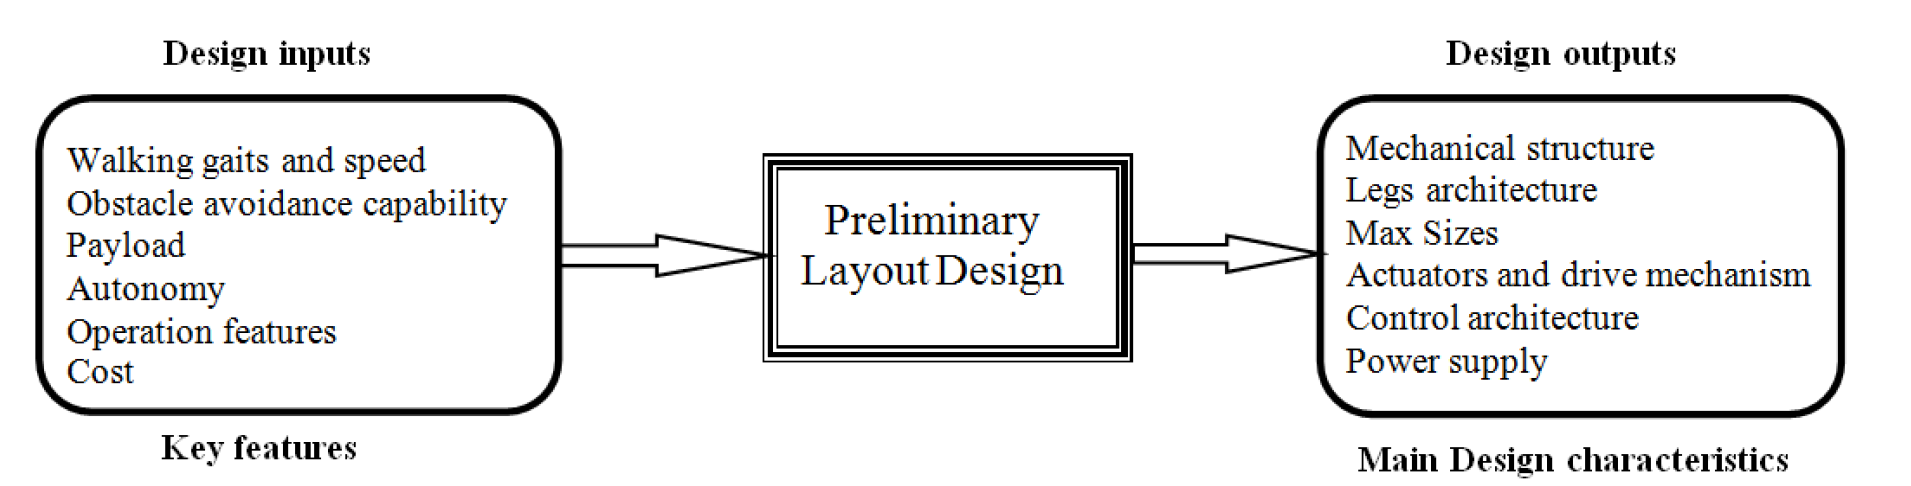
\includegraphics[width =.9\textwidth]{GD}
    \caption{ A scheme for preliminary layout design of hexapod walking robots.}
	\label{GD}
\end{figure}

\section{Hardware overview}
ZagHexa is a hexapod robot with 18 DOFs (three degrees of freedom (DOF) for each leg), it can walk in any direction (translation), or turn in place (rotation), or any combination of the two. The leg lift and ride height is adjustable as well. The robot uses a distributed walking control system based on the neurobiology of insects, stepping in the sagittal plane to angled stepping, which then induces turning in the robot.
It is an integrated multi-legged walking robot based on de-facto standard Robotic Operating System (ROS) that employs novel and different walking patterns.
Our robot is teleoperated using hand-held devices such as a smart phone or tablet or a wireless joystick (see Fig.\ref{fig4}). Furthermore, it has its own navigation system and a camera for instant video recording and streaming.
The power to the entire system is supplied through two 5 volts NiMH batteries. There is an additional power bank to power up the Raspberry Pi and other electronic components. 

\begin{figure}[H]
	\centering
	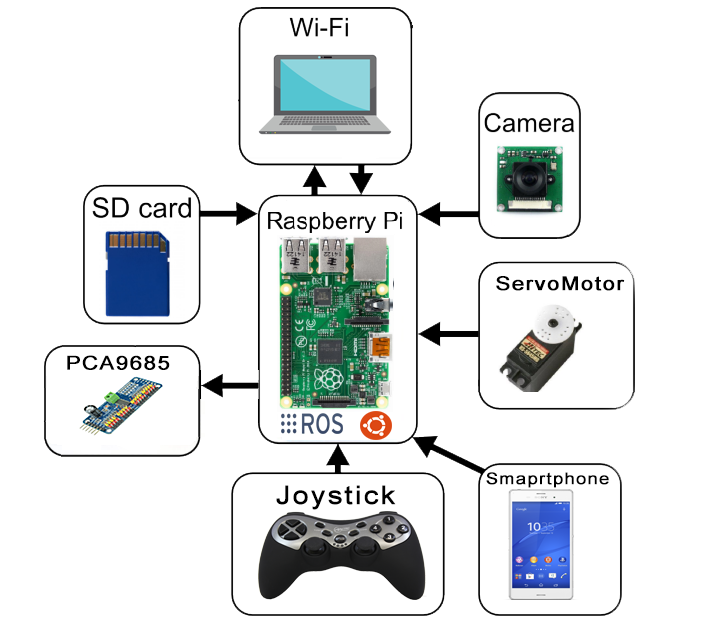
\includegraphics[width =.6\textwidth]{Fig2}
	\caption{ The electronic system of the robot.}
	\label{fig4}
\end{figure}

The final design of the ZagHexa robot constructed mainly with acrylic is shown in Fig.\ref{fig1}. ZagHexa body moves independently of its ground contact points. To make its center of gravity shift on a horizontal plane, forward/backward, and sideways moving functions are effective. These functions can also produce a smooth body movement independently of intermittent leg traveling. The robot has been designed with three degrees of freedom in the front, middle and rear legs respectively. The physical specifications are given in Table 2.
\begin{center}
\begin{tabular}{|c|c|}
    \hline
    Parameter       &       Description        \\ \hline
    Length         &           30cm           \\ \hline
    Width         &           27cm           \\ \hline
    Height         &           17cm           \\ \hline
    Weight         &           3Kg            \\ \hline
    Construction Material &                          \\ \hline
    Actuators       &     DC servo motors      \\ \hline
    Motion Control     & Servo Sequential Control \\ \hline
    Leg Stroke (Max)    &           6cm            \\ \hline
    Leg Lift (Max)     &           5cm            \\ \hline
\end{tabular}
\end{center}
\noindent
%Mechanical design
\section{Mechanical design}
\noindent In this section we will discuss the different designs of the robot including early ones as well as the final one.
\subsection{Micro ZagHexa}
We started by making a small hexapod with 18 micro servos to test our basic functions and walking algorithms. The basic parts of Micro ZagHexa is made of a 1 mm thick Aluminium sheet.

\begin{figure}[H]
	\centering
	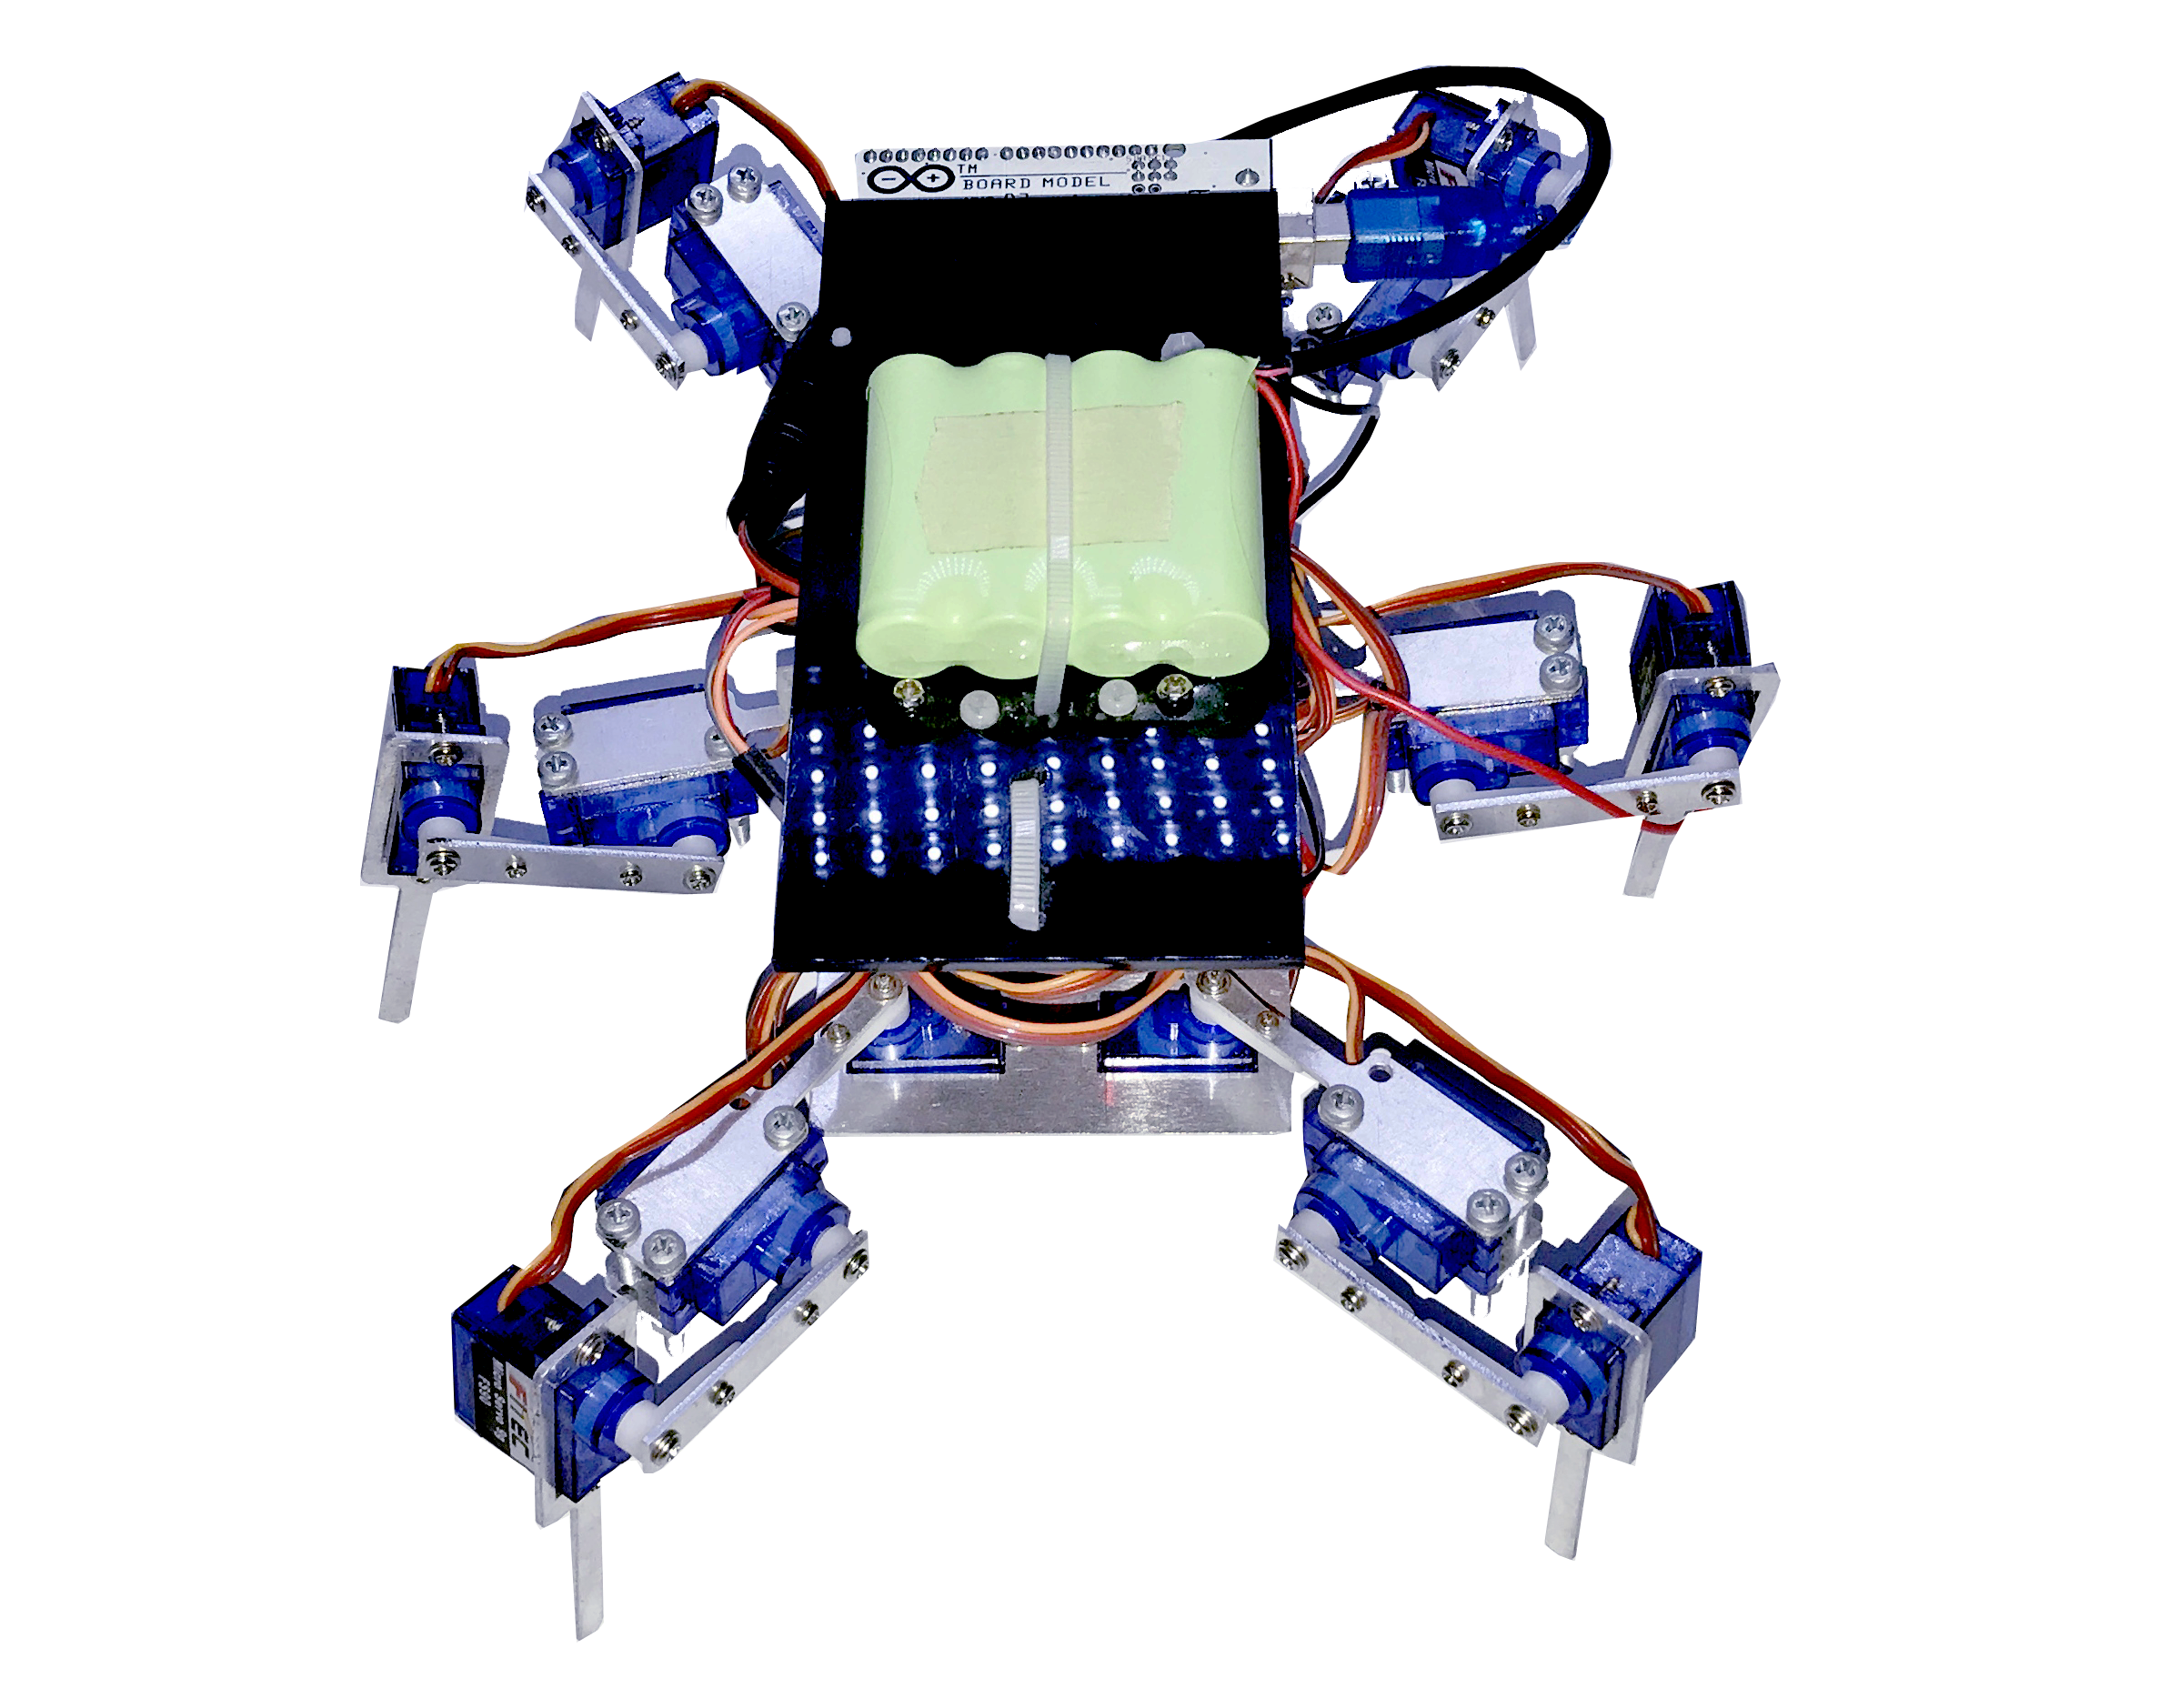
\includegraphics[width=5cm,height=5cm]{figures/uZagHexaFinal.png}
	\caption{Micro ZagHexa}
	\label{figure_i}
\end{figure}

\subsection{ZagHexa}
We moved to our next hexapod design and made it bigger and more natural looking with an articulate leg and body design. ZagHexa is made of 2.5 mm thick Acrylic. \ref{figure_} shows the CAD model of Zaghexa and \ref{figure_} shows it after being assembled.
%\begin{figure}[h]
%	\centering
%	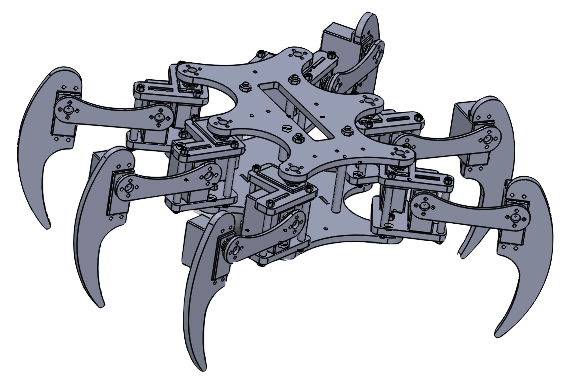
\includegraphics{figure_j}
%	\caption{CAD model of ZagHexa}
%	\label{figure_j}
%\end{figure}
\begin{figure}[H]
	\centering
	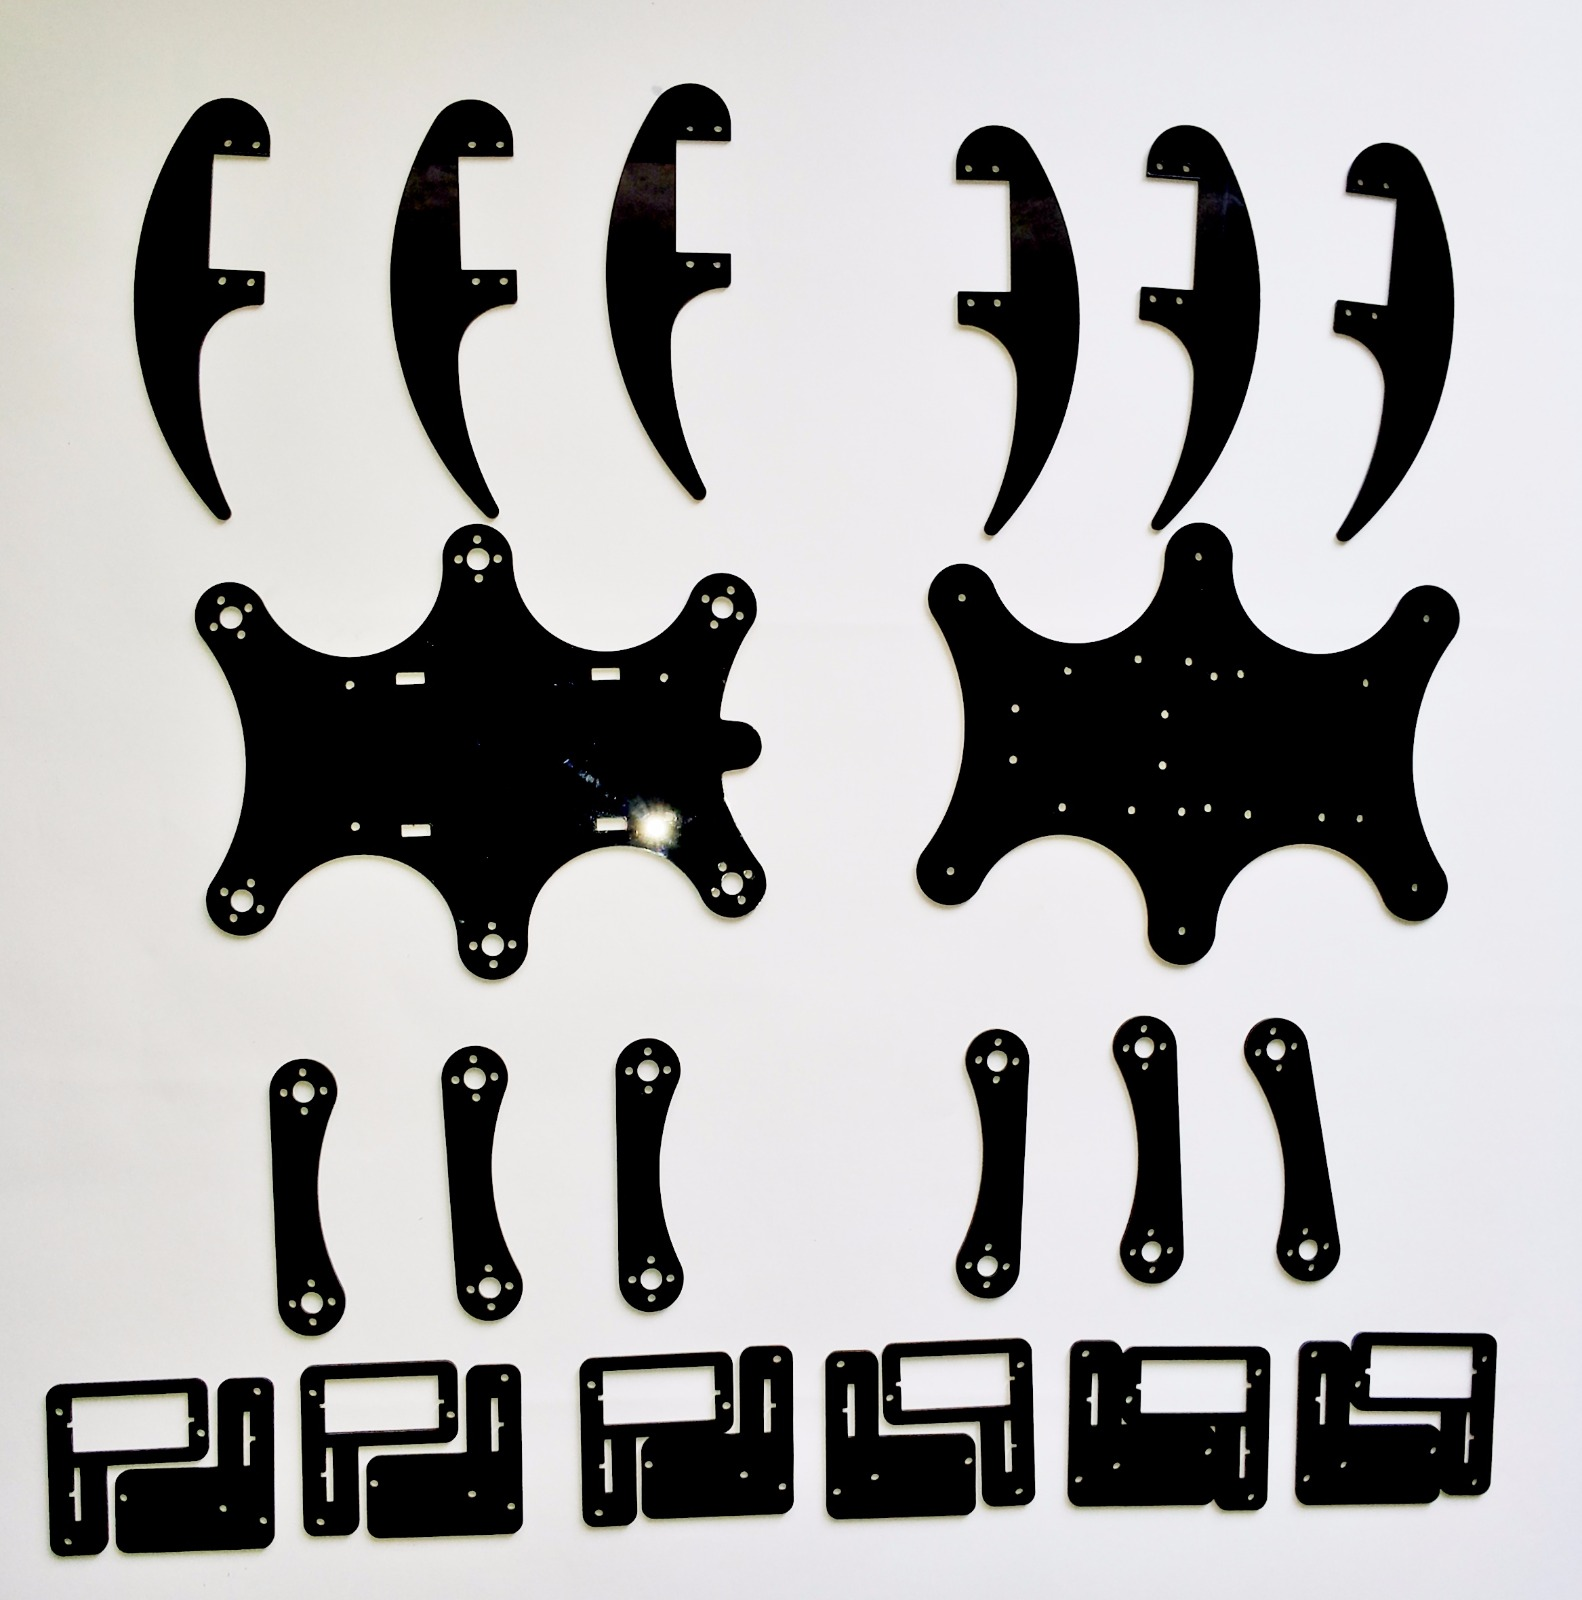
\includegraphics[width=10cm,height=11cm]{figure_k}
	\caption{ZagHexa during assembling}
	\label{figure_k}
\end{figure}
\begin{figure}[H]
	\centering
   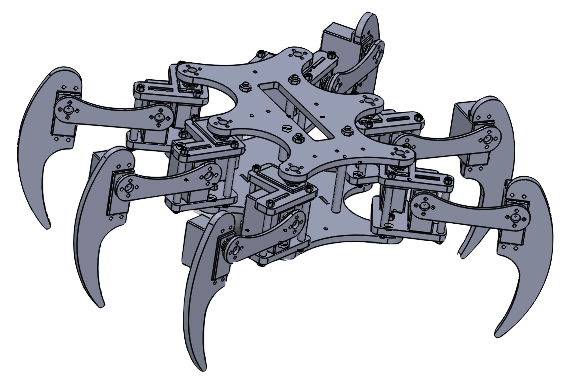
\includegraphics[width=0.45\textwidth]{figure_j}
	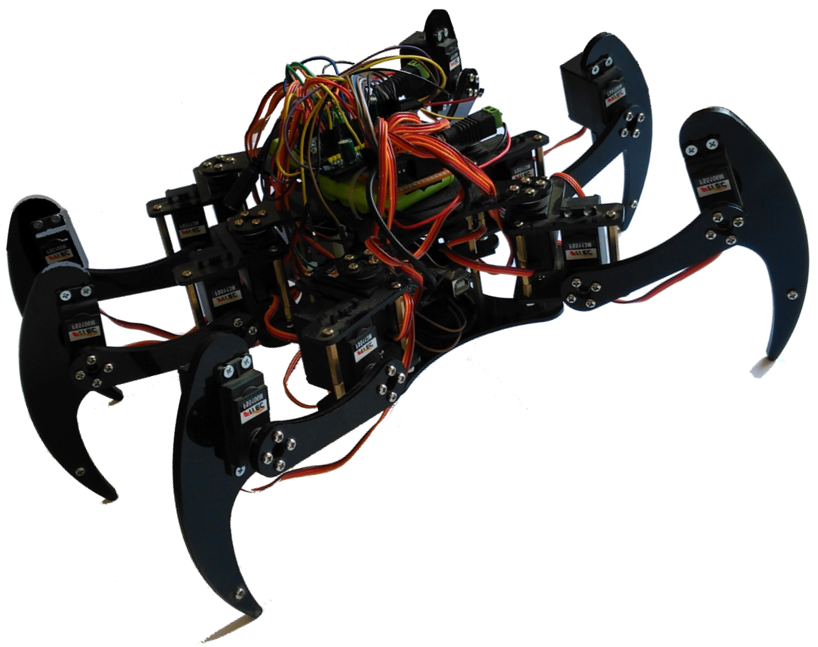
\includegraphics[width=0.45\textwidth]{Fig12}
	\caption{CAD model (left) and assembled ZagHexa (right)}
	\label{figure_l}
\end{figure}

\subsection{Giant ZagHexa}
Lastly, we made the giant version of our hexapod. It is made of a double layer 1 mm thick Aluminium sheet. The CAD model of Giant ZagHexa is shown in \ref{figure_m} and \ref{figure_o} shows it after assembling.
\begin{figure}[H]
	\centering
	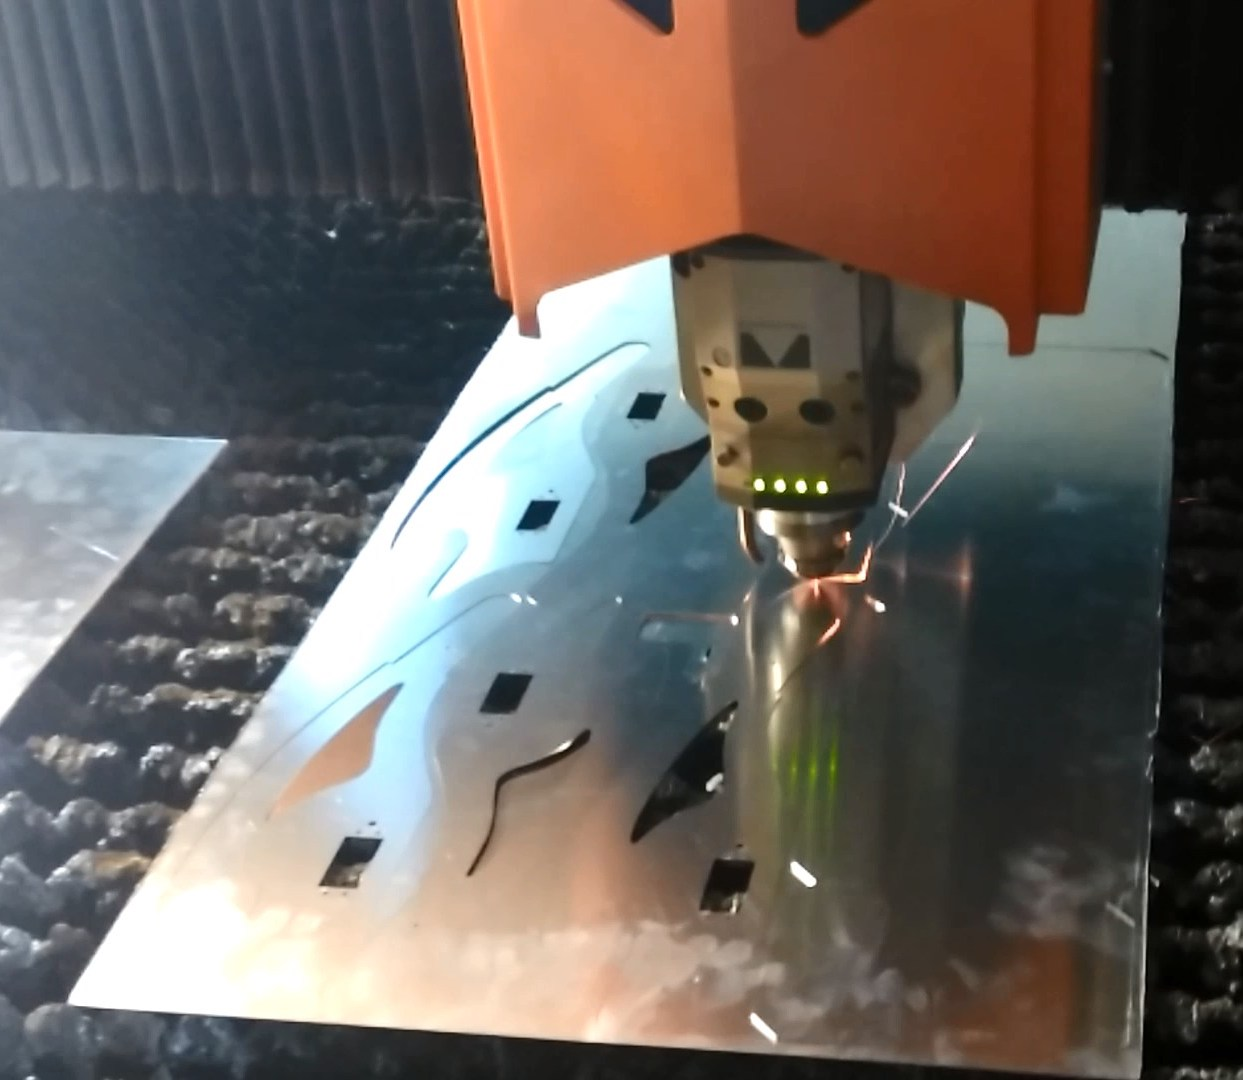
\includegraphics[width=0.7\textwidth]{figure_n}
	\caption{Giant ZagHexa during laser cutting}
	\label{figure_n}
\end{figure}
\begin{figure}[H]
	\centering
    	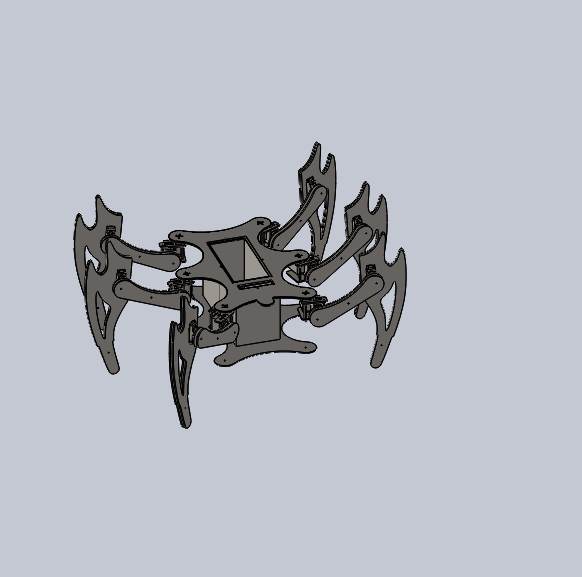
\includegraphics[width=0.45\textwidth]{figure_m}
	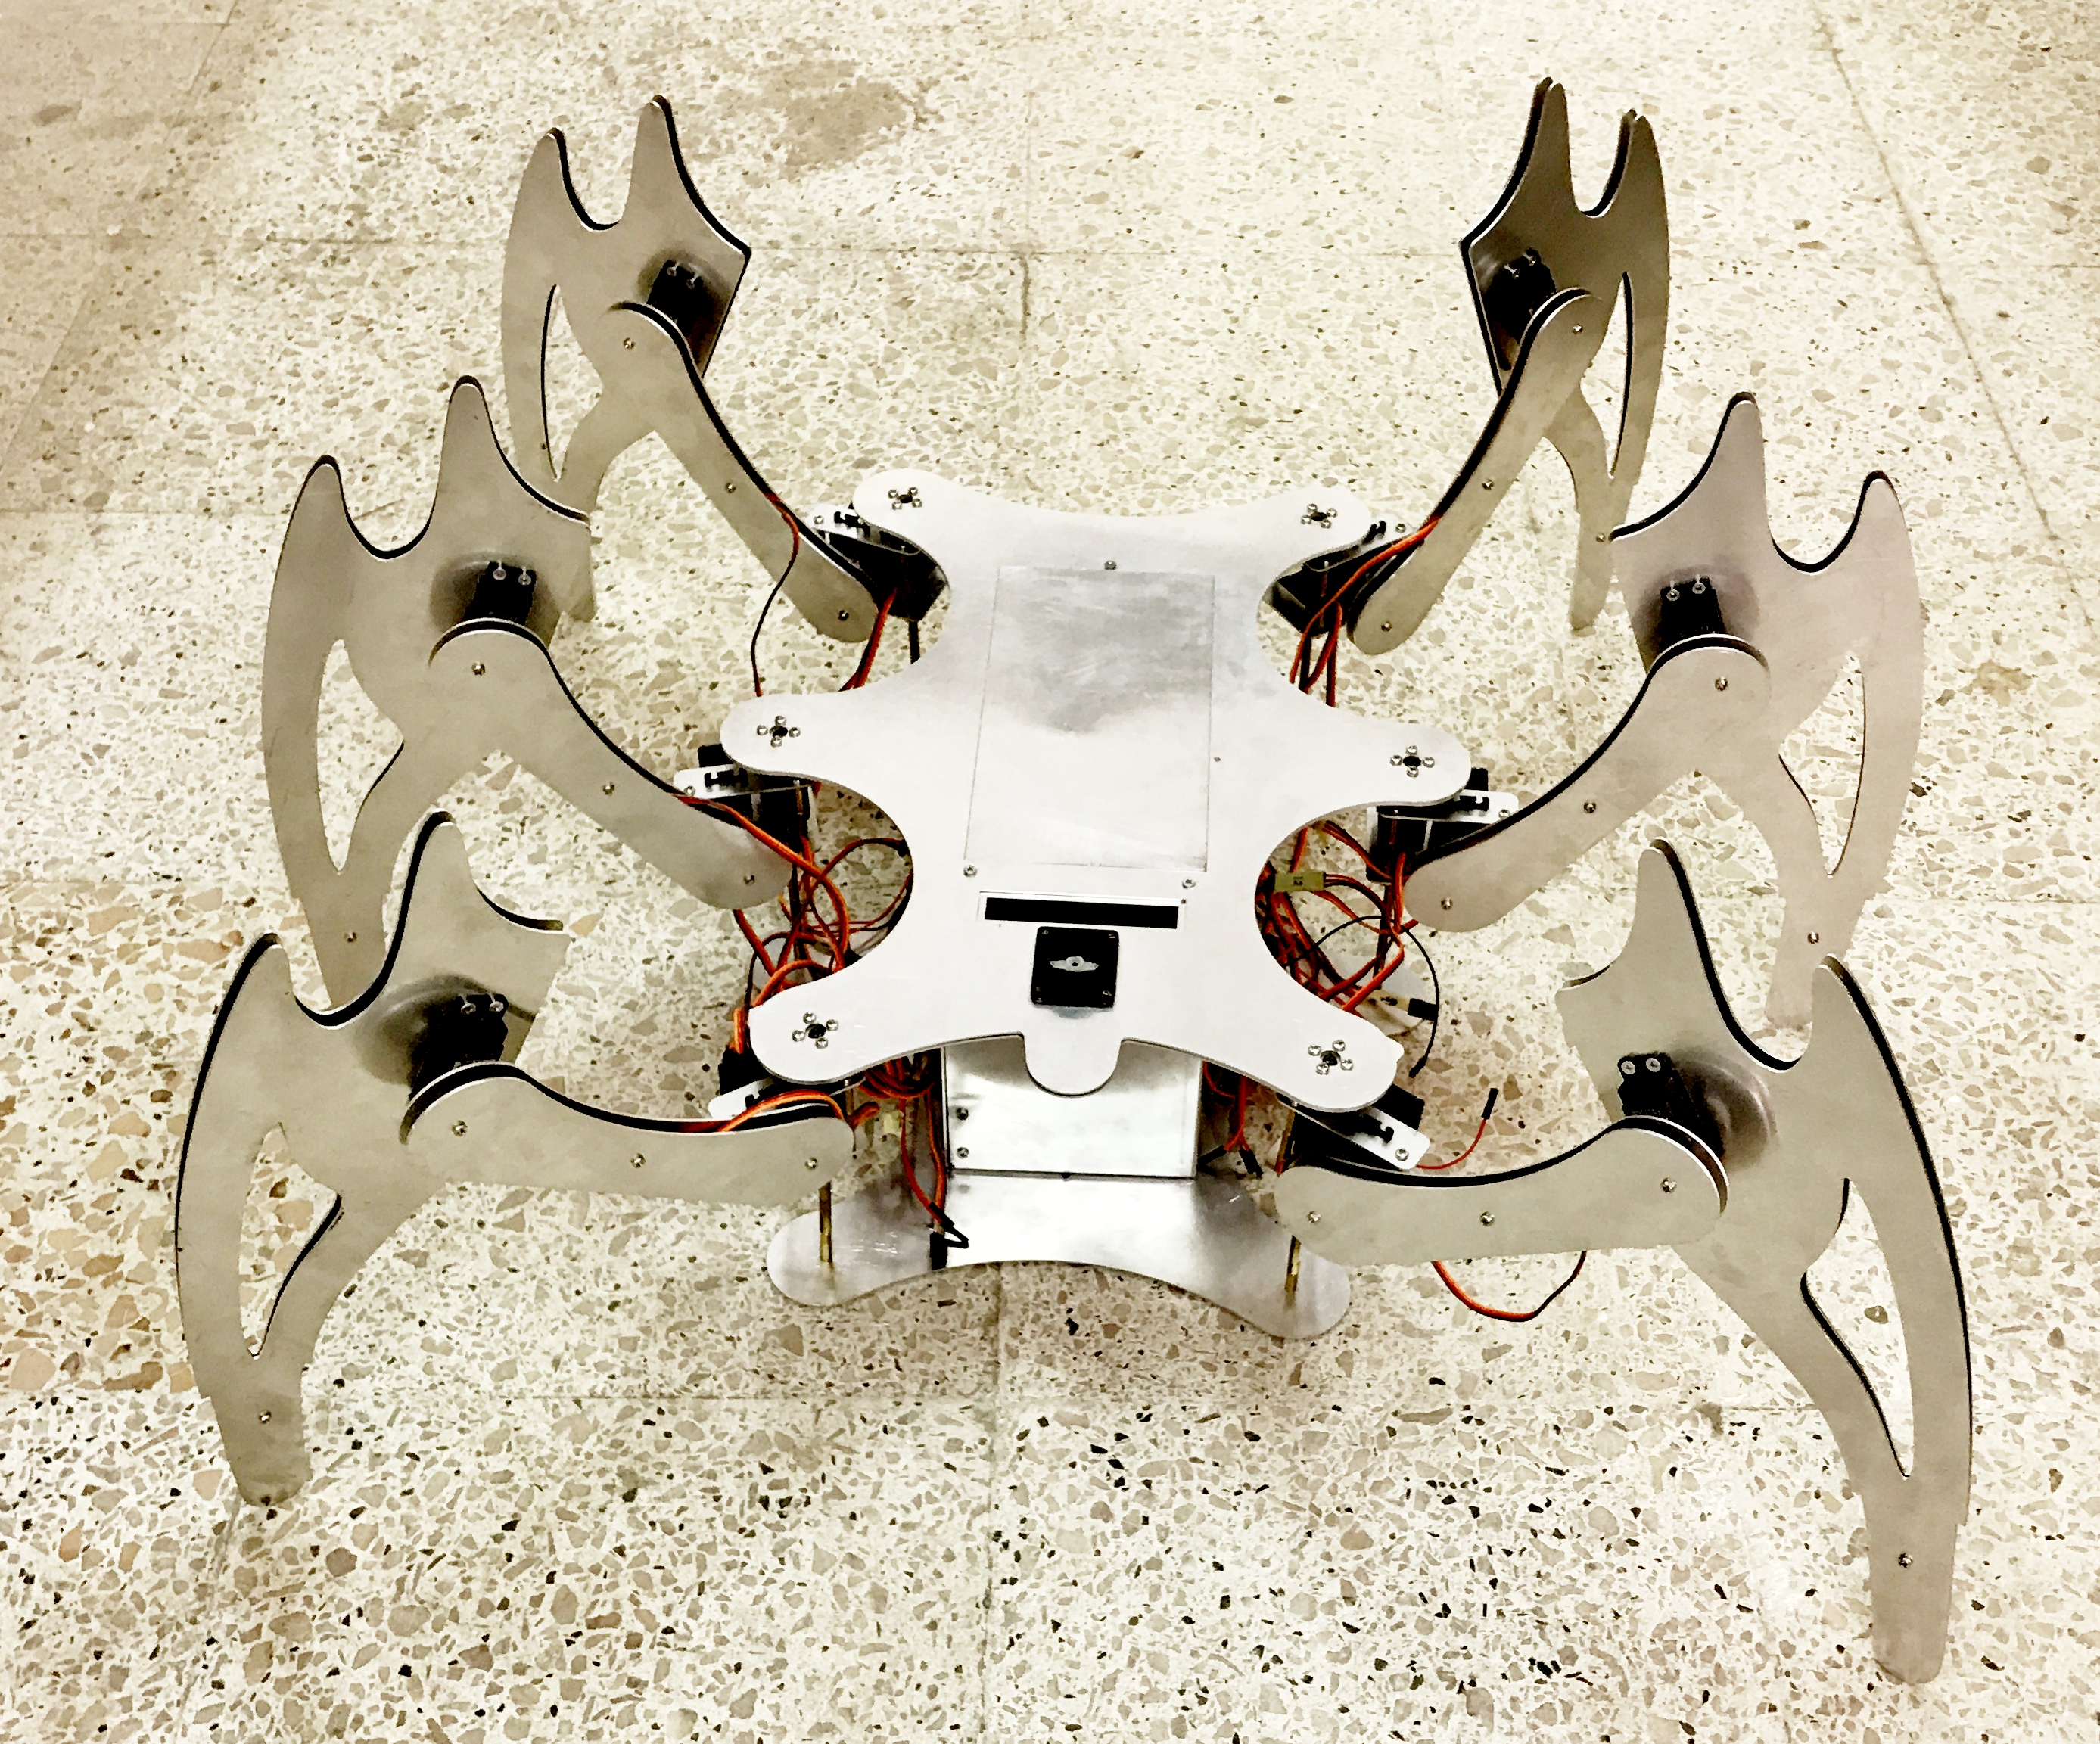
\includegraphics[width=0.45\textwidth]{figure_o}
	\caption{CAD model (left) and assembled Giant ZagHexa (right)}
	\label{figure_o}
\end{figure}


The giant ZagHexa was a little disappointing as servo motors were not strong enough to drive our hexapod. We tried to make the chassis lighter but that did not solve the problem completely. It still have stability issues.

%Electronics
\section{Electronics}
In this section we will talk about the electronic components we have been using through the whole project.
\subsection{Adafruit PCA9685}
Firstly, we used the Adafruit PCA9685 servo controller shown in \ref{figure_i} and \ref{figure_j}. Although driving servo motors with the Arduino Servo library is pretty easy, each one consumes a precious pin - not to mention some Arduino processing power.  The Adafruit 16-Channel 12-bit PWM/Servo Driver will drive up to 16 servos over I2C with only 2 pins.  The on-board PWM controller will drive all 16 channels simultaneously with no additional Arduino processing overhead.  Moreover, we can chain up to 62 of them to control up to 992 servos - all with the same 2 pins!
\begin{figure}[H]
	\centering
	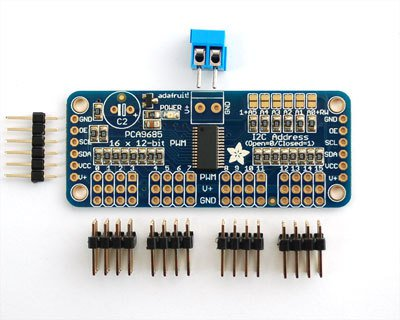
\includegraphics{figure_i}
	\caption{Adafruit PCA9685}
	\label{figure_i}
\end{figure}
\begin{figure}[H]
	\centering
	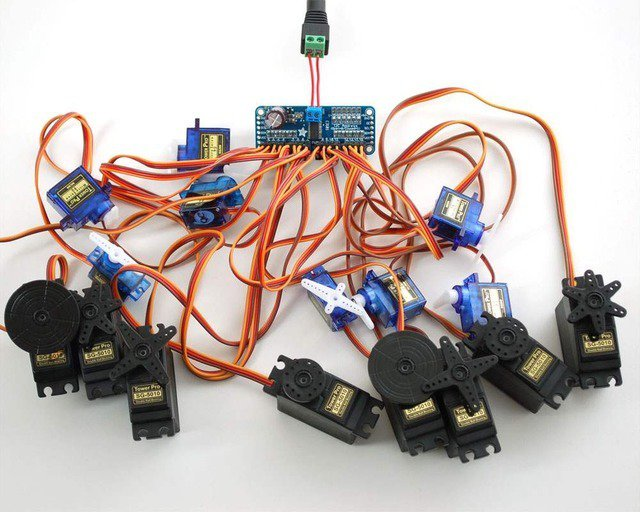
\includegraphics[width=14cm,height=10cm]{figure_p}
	\caption{Adafruit PCA9685 wiring}
	\label{figure_p}
\end{figure}
\subsection{Servo Motors}
We used 18 servo motors of different sizes as actuators. A 7 kg.cm servo motor is used to drive the tibia part as well as the coxa. The motor that will lift the whole leg should be much stronger so we used a 13 kg.cm servo. That's it, we have 3 servo motors in each leg(3 DOFs): one for coxa and one for tibia and a stronger one for the femur.

\begin{figure}[H]
	\centering
	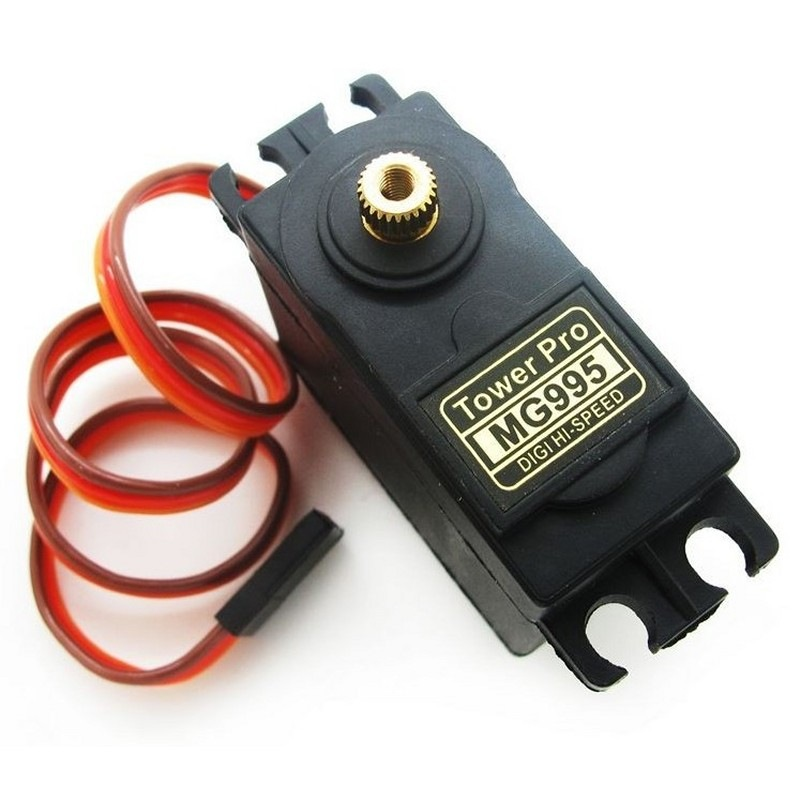
\includegraphics[width=7cm,height=5cm]{figure_q}
	\caption{13 kg.cm servo motor}
	\label{figure_q}
\end{figure}

\subsection{Playstaion joystick}
In earlier versions of ZagHexa, we used a wireless playstation 2 controller to teleoperate the hexapod. It communicates with the arduino through its uniqe via an SPI communication protocol.

\begin{figure}[H]
	\centering
	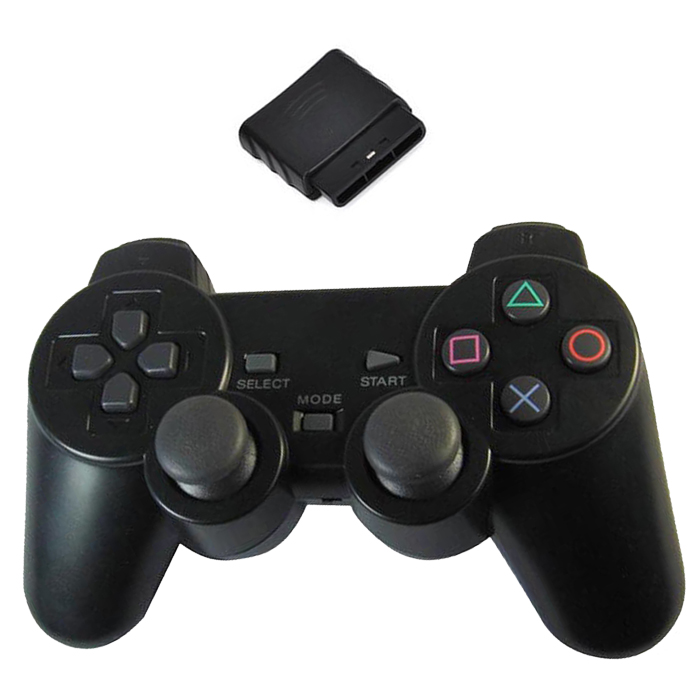
\includegraphics[width=4.0cm,height=4.0cm]{figure_r}
	\caption{Playstaion 2 controller}
	\label{figure_r}
\end{figure}

\subsection{PS2/Serial converter}
A converter is used to keep the communication between the joystick and the controller happens serially so it well be easier to handle.

\begin{figure}[H]
	\centering
	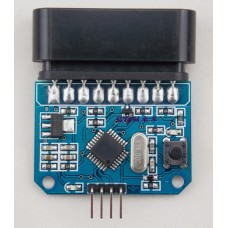
\includegraphics[width=4cm,height=6cm]{figure_s}
	\caption{PS2/Serial adapter}
	\label{figure_s}
\end{figure}

\subsection{Arduion Mega}
Later, we use an Arduino Mega in replacement of the PCA 9685 servo controller to send PWM signals to each servo motor. The reason why we moved our work from the servo controller to the Arduino Mega is that the servo controller can NOT withstand voltage above 6 Volts nor current above 5 Amps.

\begin{figure}[H]
	\centering
	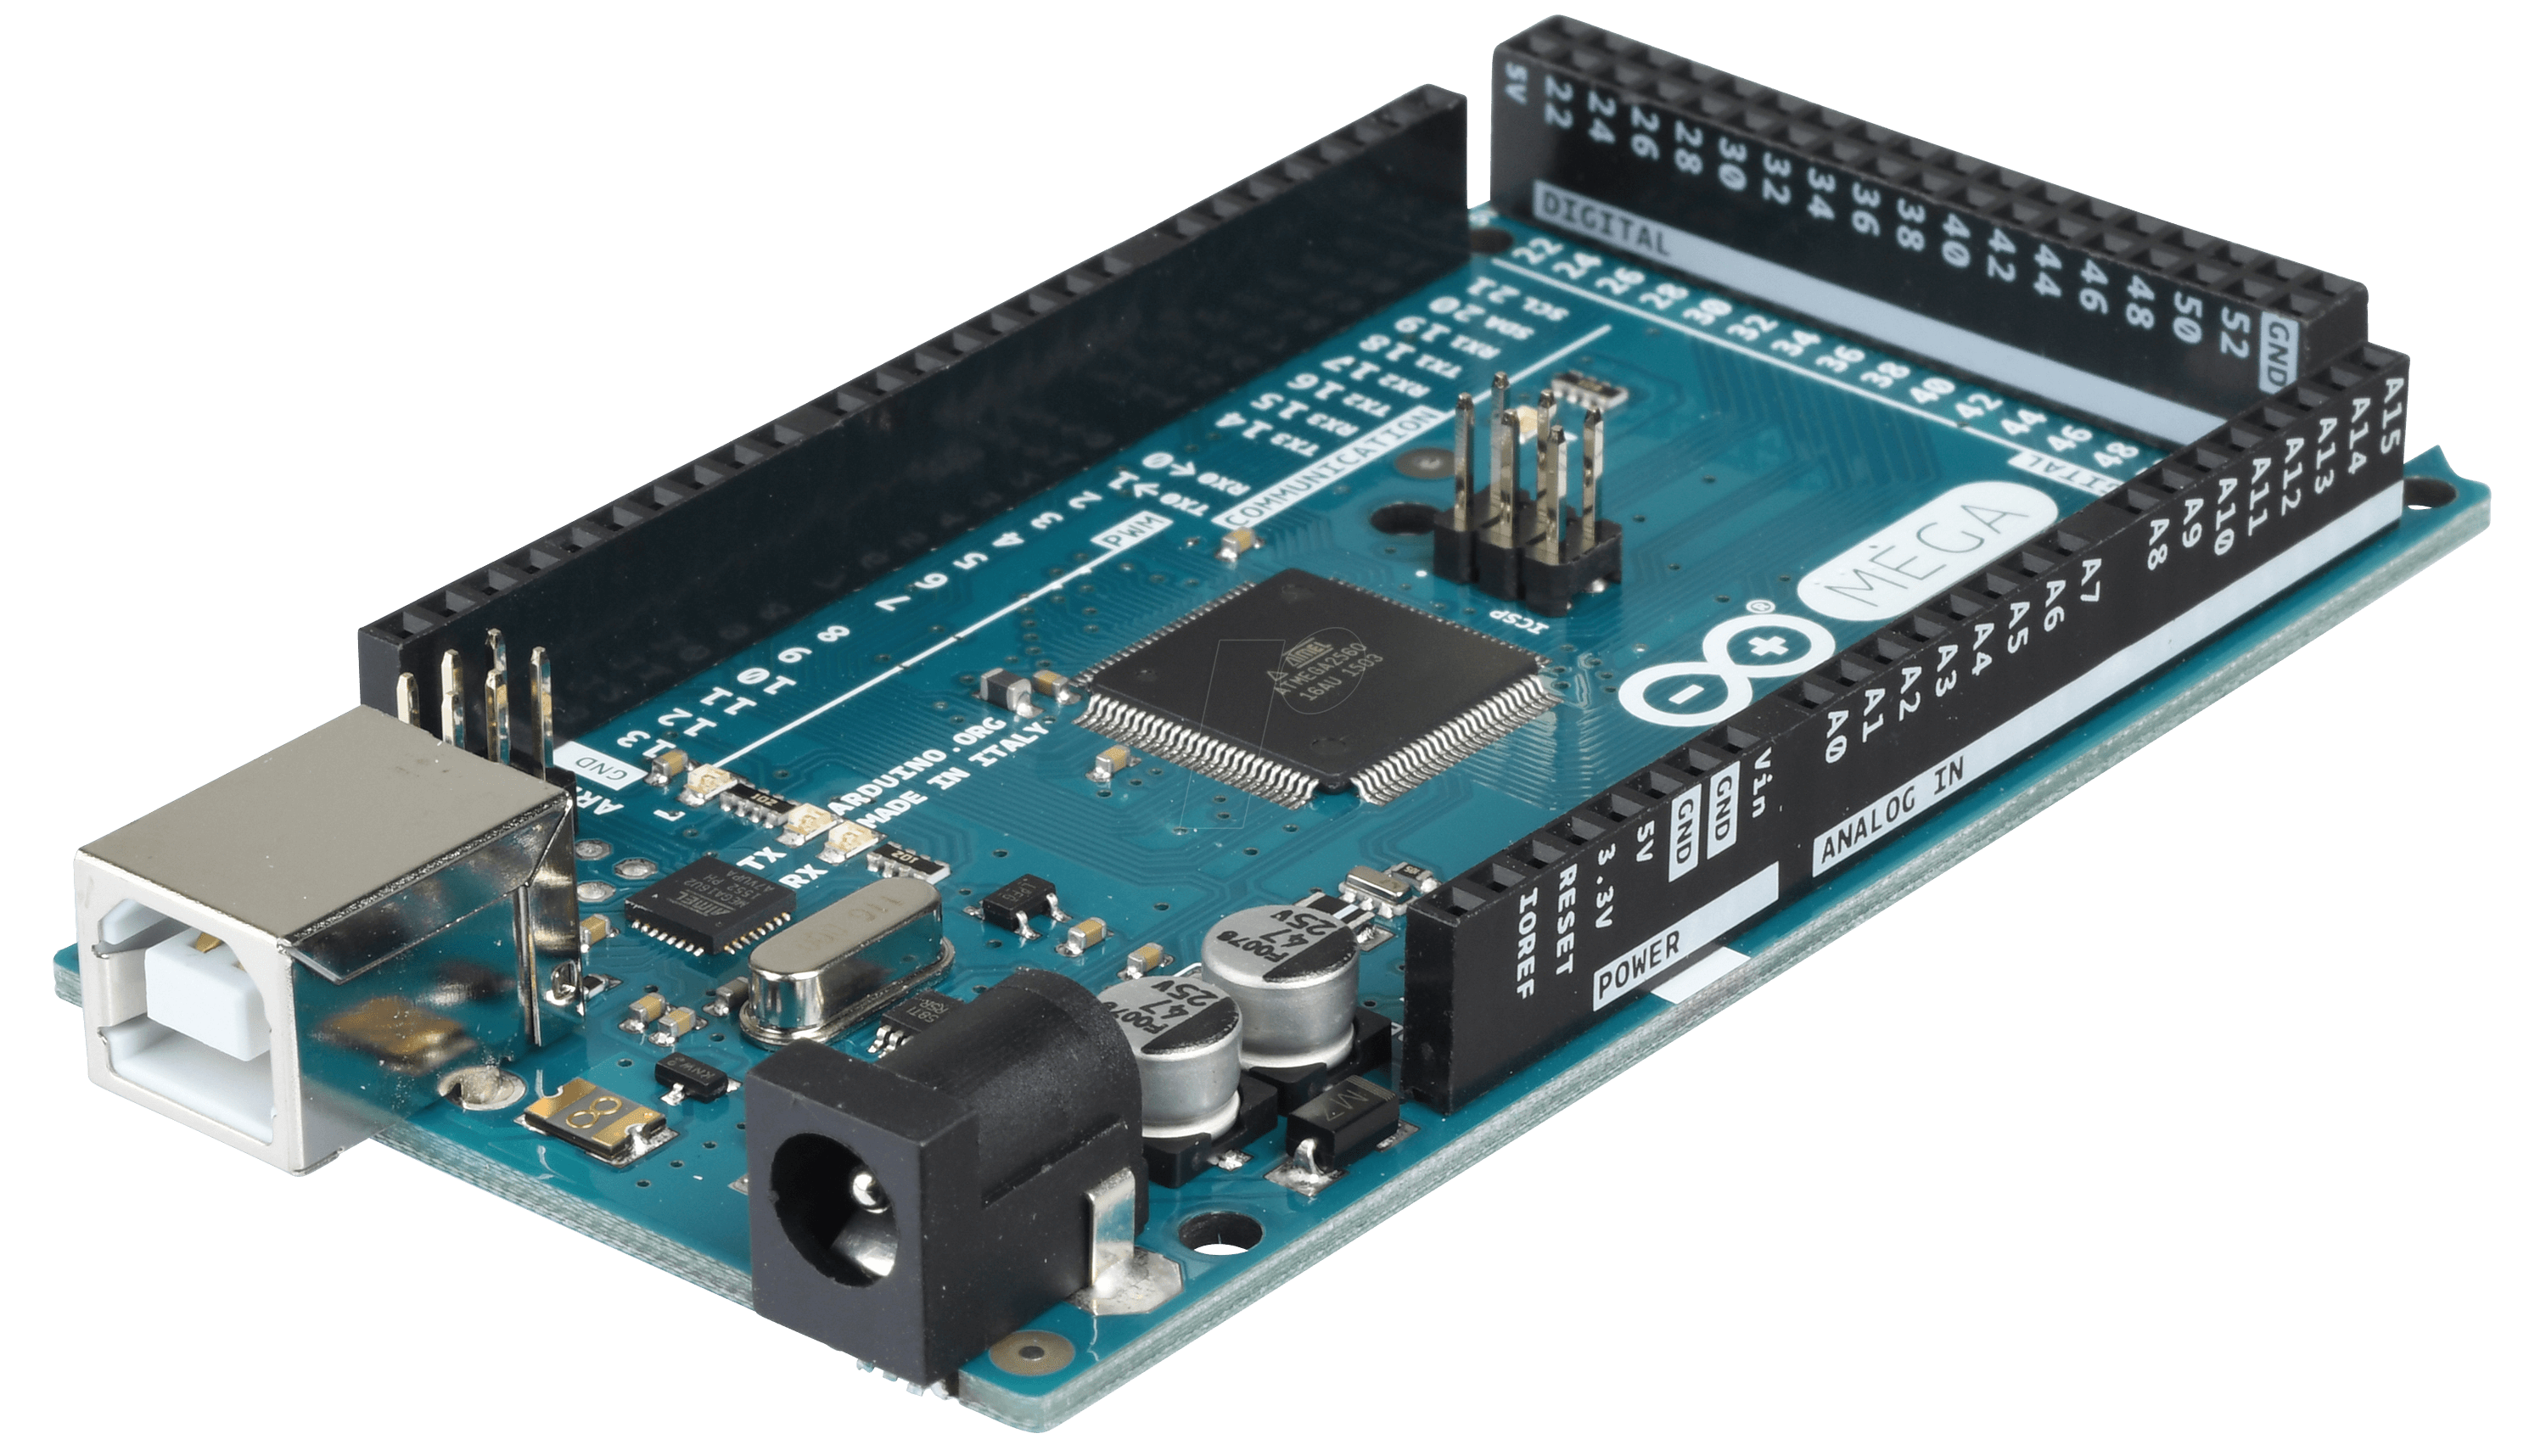
\includegraphics[width=14cm,height=10cm]{figure_t}
	\caption{Arduino Mega 25600}
	\label{figure_t}
\end{figure}

	 Arduino Mega specification
\begin{center}
	\begin{tabular}{ |c|c|}
		\hline
		Microcontroller			& ATmega2560 \\ \hline
		Operating Voltage		& 5V\\ \hline
		Input Voltage			& (recommended) 7-12V\\ \hline
		Input Voltage (limits) 	& 6-20V\\ \hline
		Digital I/O Pins 		& 54 (of which 14 provide PWM output)\\ \hline
		Analog Input Pins 		& 16\\ \hline
		DC Current per I/O Pin	& 40 mA\\ \hline
		DC Current for 3.3V Pin & 50 mA\\ \hline
		Flash Memory			& 256 KB of which 8 KB used by bootloader\\ \hline
		SRAM					& 8 KB\\ \hline
		EEPROM 					& 4 KB\\ \hline
		Clock Speed 			& 16 MHz\\ \hline
	\end{tabular}
\end{center}

\subsection{Servo interface}
We want to make a servo interface with the arduino mega and that would make installing the servos so easy without making a mess. In theory we could use 48 servos on a Mega board, but we only soldered 18 servo ports, just to keep wires tidy and compact.

\begin{figure}[H]
	\centering
	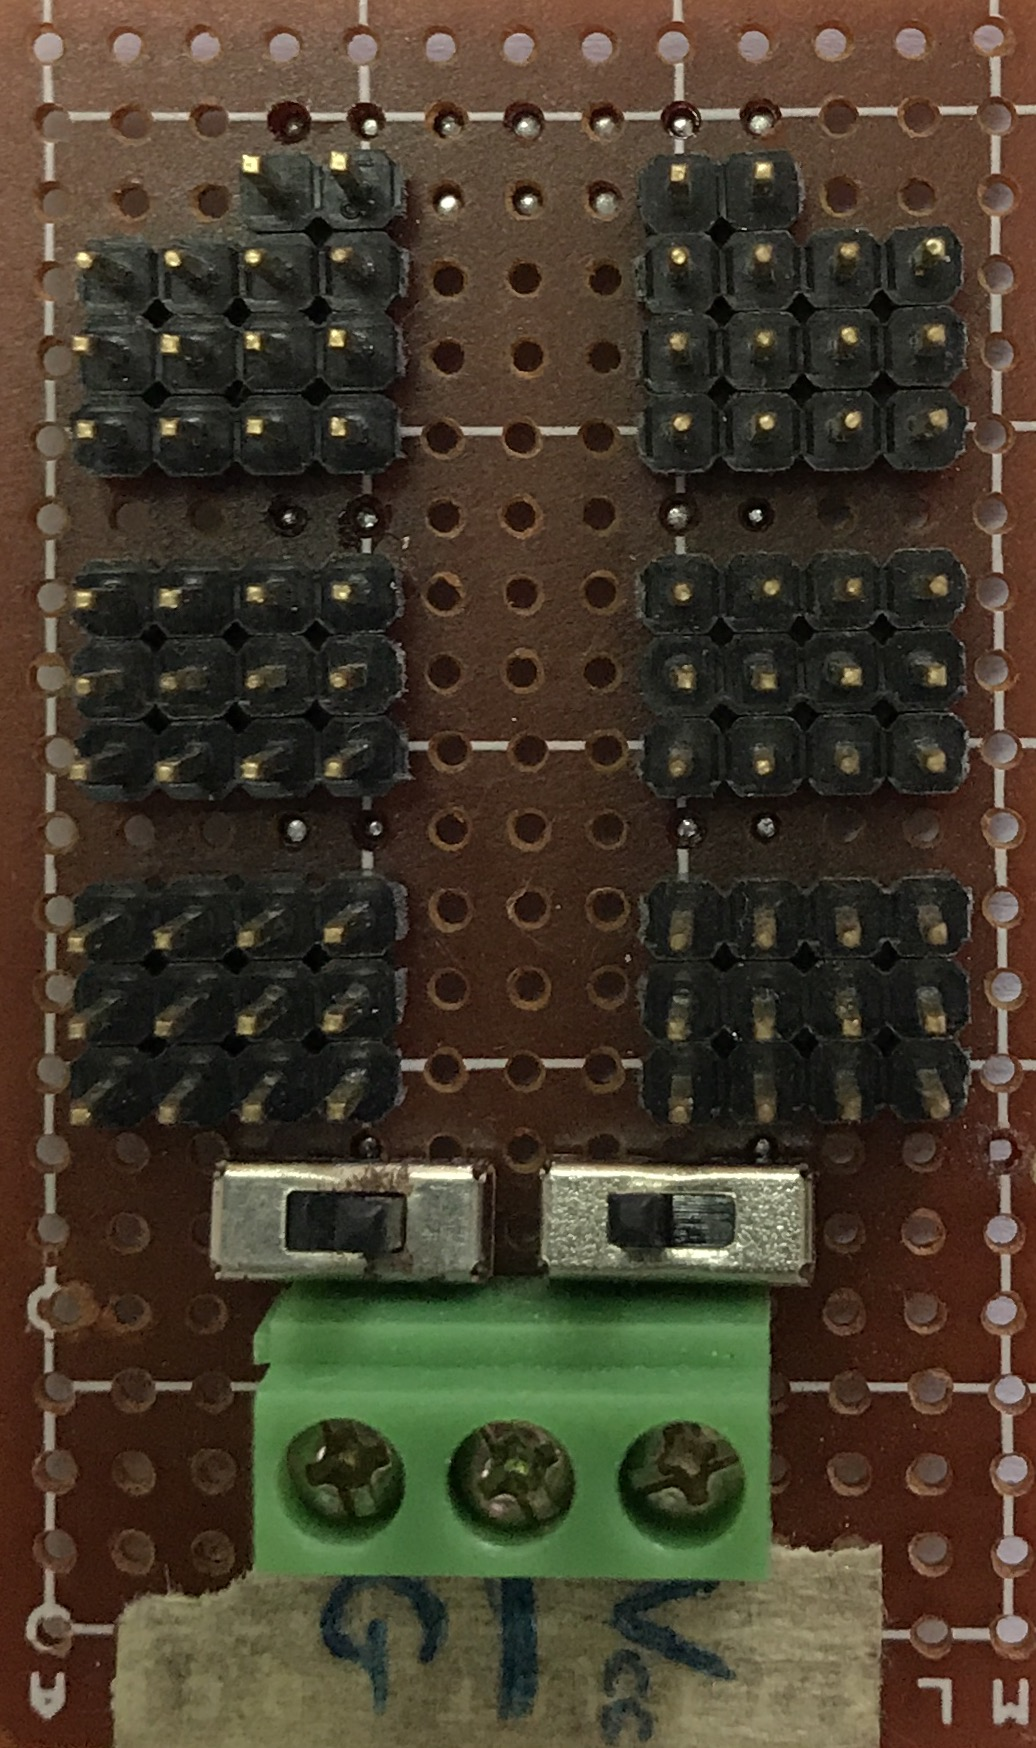
\includegraphics[width=4cm,height=6cm]{figure_u}
	\caption{Servo interface}
	\label{figure_u}
\end{figure}

\subsection{Raspberry Pi 3}
We used a Raspberry Pi 3 as an embedded computer to host our OS and to run ROS (Robotic Operating System). With the folllowing specs, Raspberry Pi is a very good choice for an embedded PC besides offering a set of GPIO pins as well.

\begin{figure}[H]
	\centering
	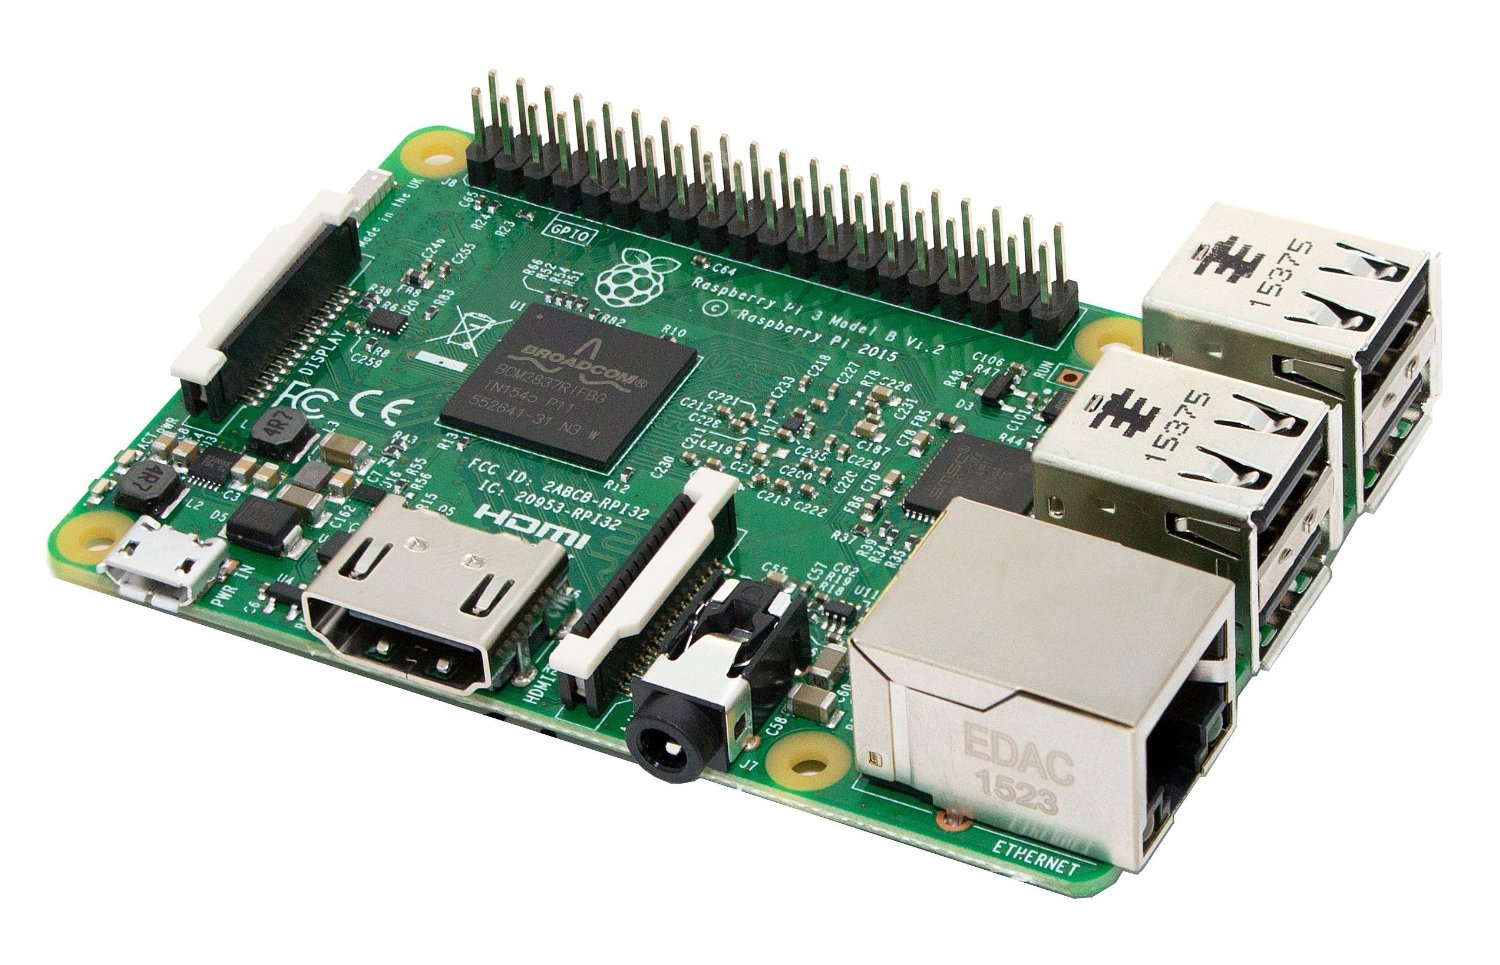
\includegraphics[width=9cm,height=5cm]{figure_v}
	\caption{Raspberry Pi 3 model B}
	\label{figure_v}
\end{figure}
\begin{center}
\begin{tabular}{ |l||p{12cm}|}
	\hline
	Processor      & Broadcom BCM2387 chipset. 1.2GHz Quad-Core ARM Cortex-A53 802.11 b/g/n Wireless LAN and Bluetooth 4.1 (Bluetooth Classic and LE)\\ \hline
	GPU               & Dual Core VideoCore IV® Multimedia Co-Processor. Provides Open GL ES 2.0, hardware-accelerated OpenVG, and 1080p30 H.264 high-profile decode. \\ \hline
	Memory          & 1GB LPDDR2  \\ \hline
	Operating System  & Boots from Micro SD card, running a version of the Linux operating system  \\ \hline
	Dimensions     & 85 x 56 x 17mm  \\ \hline
	Power             & Micro USB socket 5V1, 2.5A  \\ \hline
	Ethernet          & 10/100 BaseT Ethernet socket  \\ \hline
	Video Output   & HDMI (rev 1.3 \& 1.4 Composite RCA (PAL and NTSC)  \\ \hline
	Audio Output   & Audio Output 3.5mm jack, HDMI     \\ \hline
	USB                 & 4 x USB 2.0 Connector   \\ \hline
	GPIO Connector    & 40-pin 2.54 mm (100 mil) expansion header: 2x20 strip Providing 27 GPIO pins as well as +3.3 V, +5 V and GND supply lines \\ \hline
	Camera Connector  & 15-pin MIPI Camera Serial Interface (CSI-2) \\ \hline
	Display Connector & Display Serial Interface (DSI) 15 way flat flex cable connector with two data lanes and a clock lane    \\ \hline
	Memory Card       & Slot Push/pull Micro SDIO  \\ \hline
\end{tabular}
\end{center}


\subsection{NIMH battery}
We used a 5 volts NIMH battery to power up servo motors. With 1500 mAh capacity, ZagHexa is able to run for about 15 minutes.

\begin{figure}[H]
	\centering
	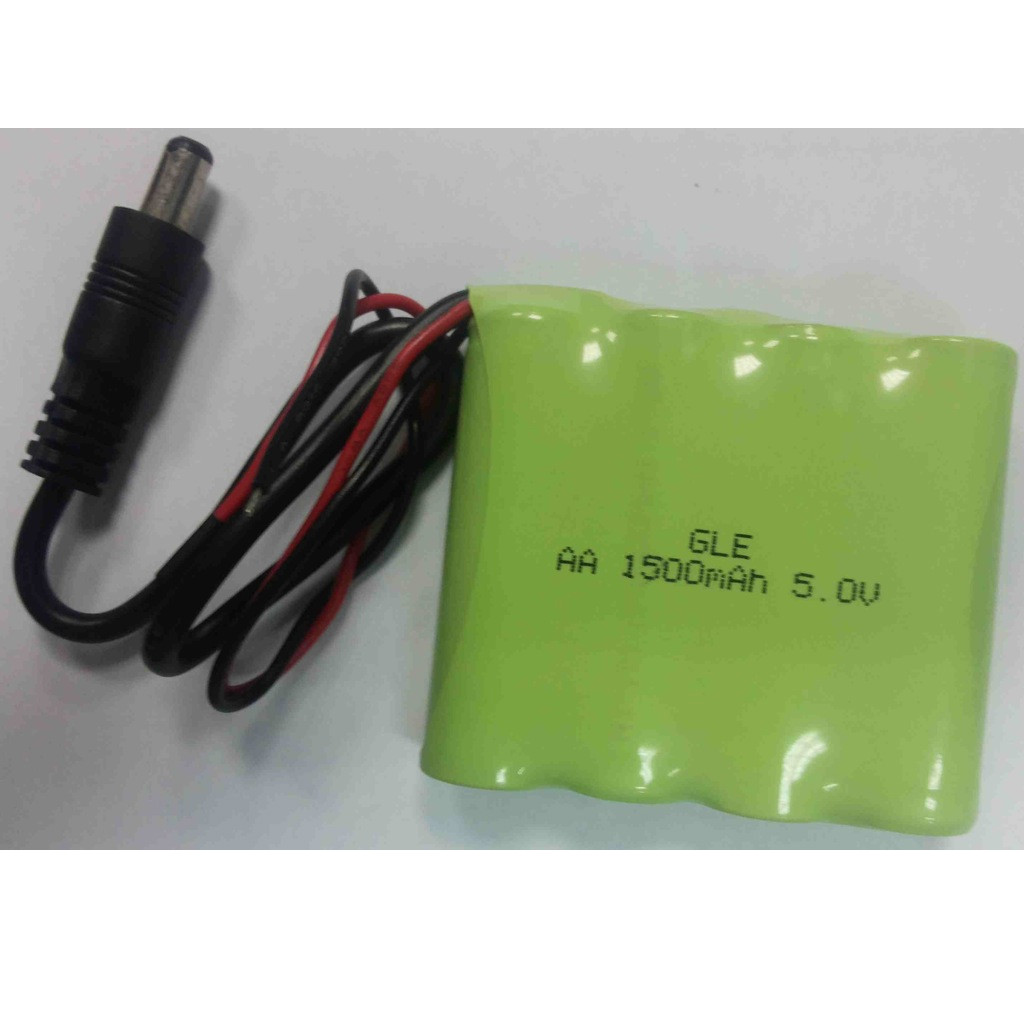
\includegraphics[width=8cm,height=5cm]{figure_w}
	\caption{5V NIMH battery}
	\label{figure_w}
\end{figure}